\chapter{Measurement of \texorpdfstring{$\thetaot$}{theta13}}
\label{ch:analysis}

The 3-flavor model of neutrino oscillation discussed in \cref{ch:intro}
was tested for goodness-of-fit against the Daya Bay observations,
and best-fit values for the oscillation parameters \thetaot{} and \dmee{}
were extracted.
For a \nuebar{} with energy $E_\nu$,
the probability that it will be detected as a \nuebar{}
after traveling a distance $L$ is predicted in the 3-flavor model as:

\begin{align}\label{eq:p_sur}
    \begin{split}
        P_\text{sur} = 1 &- \cos^4\thetaot\sin^22\theta_{12}\sin^2\Delta_{21} \\
                         &- \sin^22\thetaot(\cos^2\theta_{12}\sin^2\Delta_{31}
                     + \sin^2\theta_{12}\sin^2\Delta_{32}) \\
        \simeq 1 &- \cos^4\thetaot\sin^22\theta_{12}\sin^2\Delta_{21} \\
                 &- \sin^22\thetaot\sin^2\Delta_{ee},
\end{split}
\end{align}
where
$\Delta_{ji} \simeq 1.267 \Delta m^2_{ji} (\si{\eV}^2) L(\si{\m})/E_\nu (\si{\MeV})$,
and
$\Delta m_{ee} \simeq \cos^2\theta_{12}\left|\Delta m^2_{31}\right| +
\sin^2\theta_{12}\left|\Delta m^2_{32}\right|$.
As described in detail in \cref{ch:intro},
the use of $\Delta m^2_{ee}$ to model the Daya Bay observations
is appropriate since the measurement is not sensitive
to the $O(\SI{1}{\percent})$ difference between $\Delta m^2_{31}$ and $\Delta m^2_{32}$.
Either form of \cref{eq:p_sur} can be used to compute the \nuebar{} survival probability
from the Daya Bay reactors to the near and far halls,
and this analysis uses the full 3-flavor form.
%Values for the physical mass-squared differences will be computed
%based on the extracted value of $\Delta m^2_{ee}$.

To assess the validity of the 3-flavor model and extract the oscillation parameters'
best-fit values,
a comparison was made between the observed near-site and far-site \nuebar{} spectra.
The comparison relies on the number of observed events at the near halls (EH1 and EH2)
and $P_\text{sur}$ from the 3-flavor oscillation model
to predict the far-hall (EH3) observations
with minimal reliance on the intricacies of reactor operation modeling
and antineutrino production (\cref{sec:prediction}).
Reactor models were used in the prediction
to determine the relative \nuebar{} flux
observed by each AD from each reactor core (\cref{sec:reactor}).
A \chisquare{} expression was created to quantify the agreement
between the prediction prediction and observations (\cref{sec:fitter}).

\section{Reactor model}
\label{sec:reactor}

The relative flux and spectrum of \nuebar{} from each reactor core was used
to adjust the predicted IBD spectrum at the far-hall ADs
based on how many \nuebar{} a particular near-hall AD was exposed to,
as described in detail in \cref{sec:prediction}.
The \nuebar{} production from each reactor was estimated from 3 fundamental contributions:
emission from fission products, corrections due to non-equilibrium effects,
and emission from spent nuclear fuel (SNF).
The resulting emission spectra specifying the spectrum per fission
were combined with knowledge of reactor power, fuel composition,
and energy released per fission
to estimate the total emitted \nuebar{} spectrum from each core.

The \nuebar{} spectrum is estimated for each of the four main fission isotopes
(\isotope[235]{U}, \isotope[238]{U}, \isotope[239]{Pu}, and \isotope[241]{Pu})
using the Huber and Muller models\todo{cite / more on reactor spectrum}.
Weekly average fission fractions and power levels for each core
are obtained from the power company.
The energy emitted per fission for each isotope is estimated from
[insert model].\todo[inline]{Decide which thermal energy per fission to use}
Corrections due to nonequilibrium effects, $c^{\text{ne}}$,
and spent nuclear fuel, $S^{\text{snf}}$
are estimated by .\todo{include more on noneq. and snf}
Therefore, for each week, the total number of antineutrinos
of a given energy emitted from each core can be computed,
given knowledge of a particular AD's livetime.
The total livetime of each AD for each week is computed
(ignoring the muon veto, which was corrected for in
\cref{eq:near_hall_bg_eff}).
The total expected number of \nuebar{}'s produced by core $k$
during the livetime of AD $i$ is therefore
\begin{equation}\label{eq:reactor_spectrum}
    \phi_{ik}(E) = \sum_{\text{weeks }w}
        \frac{W_{\text{th},w}}{\sum_q f_{q,w} e_q}
        \sum_{\substack{\text{isotopes}\\q}}
        f_{q,w} S_q(E) c_{q,w}^{\text{ne}} + S_w^{\text{snf}}.
\end{equation}

\section{Projection from near halls to far hall}
\label{sec:prediction}

The Daya Bay experiment was configured to use
identically-designed antineutrino detectors (ADs) at near and far sites
so that the measurements of the near and far ADs could be directly compared
with minimal systematic uncertainty due to detection efficiency
and reactor \nuebar{} modeling.
A predictive model was designed to implement the intuitive notion
that the observations at a near-hall AD can be used to predict
the observations at a far-hall AD \cite{p12e_fitter,p14a_fitter}.
This model of ``near-far projection'' estimates the contribution of each reactor core
to a given near AD's IBD sample,
then extrapolates each core's contribution to the far hall
based on oscillation effects, AD-reactor distance (baseline),
and differences in livetime, target mass and efficiency.
An alternative class of models,
where the observations at both near and far ADs
are predicted based on a model of reactor \nuebar{} emission
in addition to oscillation effects,
has been used for both nH and nGd analyses \cite{nh2016, ngd2016}.
In this thesis, the near-far projection model is used for the first time
to extract \thetaot{} from observations of neutron capture on Hydrogen.


In the simplest configuration, with a single near observation,
a single far observation, and a single isotropic source of \nuebar,
the ratio of the number of observed far events $N_\text{f}$
to the number of observed near events $N_\text{n}$
depends on only a small set of quantities:
the detection efficiencies $\varepsilon_\text{n/f}$,
the number of target protons $N_\text{p,n/f}$,
the baselines $L_\text{n/f}$,
and the survival probability $P_\text{sur}(E_\nu, L_\text{n/f})$.
If the efficiencies, baselines, and number of target protons are well-determined,
then the near-far ratio becomes sensitive
to small changes in the survival probability via the formula \cite{ngd2016}

\begin{equation}\label{eq:near_far}
    \frac{N_\text{f}}{N_\text{n}} = \left(\frac{N_\text{p,f}}{N_\text{p,n}}\right)
    \left(\frac{L_\text{n}}{L_\text{f}}\right)^2
    \left(\frac{\varepsilon_\text{f}}{\varepsilon_\text{n}}\right)
    \left[\frac{P_\text{sur}(E_\nu, L_\text{f})}{P_\text{sur}(E_\nu, L_\text{n}}\right].
\end{equation}

In practice, the presence at Daya Bay of multiple \nuebar{} sources
located hundreds of meters apart
necessitated a more complex variant of \cref{eq:near_far}
that accounted for both the differences in reactor power and \nuebar{} spectrum over time,
and the two near halls, both of which observe \nuebar{}'s
in various stages of oscillation from all six reactor cores.
Given a set of observed IBD candidates at a near-hall AD,
the near-far projection model performs the following steps,
illustrated in \cref{fig:near_far_cartoon}:

\begin{figure}
    \missingfigure{Near-far cartoon}
    \caption{Illustration of the near-far projection procedure.}
    \label{fig:near_far_cartoon}
\end{figure}

\begin{enumerate}
    \item Subtract backgrounds from the near hall measurement
        and adjust for detection efficiencies
    \item Convert the reconstructed prompt energy spectrum
        into an estimated true \nuebar{} energy spectrum
    \item Predict the contribution of each reactor core
        to the observed \nuebar{} spectrum,
        including minor oscillation effects
    \item Extrapolate each core's contribution to the far hall ADs,
        accounting for oscillation effects and the AD-reactor baseline
    \item Convert the \nuebar{} energy back into a reconstructed energy
    \item Correct for the far AD's detection efficiency, backgrounds,
        target mass, and livetime
\end{enumerate}
The predicted spectrum at each far-hall AD can be compared
with the observed spectrum, as described in \cref{sec:fitter}.
For the rate-only analysis, a single bin of reconstructed energy is used.

In the following, the indices $i$ and $j$ refer to individual ADs,
$k$ and $l$ refer to reactor cores,
and $b$ refers to bins of reconstructed energy.

\subsection{Near-hall backgrounds and efficiencies}
\label{subsec:near_bg_eff}

The observed number of IBD candidates must be adjusted
to account for the backgrounds and efficiencies described in \cref{ch:event_selection}.
The backgrounds this analysis accounts for are
accidentals, \li{}/\he{}, fast neutrons, and \amc{}.
Efficiencies that can be measured precisely for each AD,
namely
the muon-veto livetime efficiency $\varepsilon_\mu$
multiplicity efficiency $\varepsilon_m$,
and target proton effective efficiency
$\varepsilon_{p,i}=\nicefrac{N_{p,\text{AD }i}}{N_{p,\text{EH1-AD1}}}$,
are directly accounted for,
and are listed in Table X.\todo{Tables with rates \& efficiencies}
The remaining efficiencies, listed in \cref{tab:efficiencies},
are estimated for a generic or average AD and assigned a relative uncertainty.
Since the near-far projection is a relative measurement,
only deviations of individual ADs' efficiencies from the estimated mean value
impact the final prediction.
Therefore the remaining efficiencies are accounted for
by terms which quantify that potential difference.
Given a near-hall observation of $N_{\text{cand},i}^{(b)}$ IBD candidates
and $N_{\text{bg},i}^{(b)}$ estimated backgrounds in reconstructed energy bin $b$
of AD $i$,
the predicted number of IBDs is

\begin{equation}\label{eq:near_hall_bg_eff}
    N_{\text{IBD},i}^{(b)}(\thetaot, \dmee) =
    \frac{N_{\text{cand},i}^{(b)} - N_{\text{bg},i}^{(b)}}{
        \varepsilon_{\mu,i}\varepsilon_{m,i}\varepsilon_{p,i}(1+\nu_{\varepsilon,i})
        (1 + \nu_{\text{relE},i}\cdot a_{\text{relE},i}^{(b)}(\thetaot, \dmee))
    },
\end{equation}
where $\nu_{\varepsilon,i}$ is the fractional relative difference from
the estimated average value determined in \cref{ch:event_selection}
for the detection efficiency from all sources except the prompt energy cut.
The AD-to-AD differences in prompt energy cut efficiency arise from two effects:
the distortion of the spectrum from oscillations,
and the distortion of the spectrum from differences
in relative energy scale.
The relative energy scale (\cref{subsec:rel_energyscale})
is accounted for by a separate AD-dependent parameter $\nu_{\text{relE},i}$,
the fractional deviation of a given AD's energy scale
from the nominal value assumed for all ADs.
The parameter $a_{\text{relE},i}^{(b)}(\thetaot, \dmee)$
represents the fractional change to a given bin of reconstructed energy
if the relative energy scale were to change by $1\sigma \sim \SI{+-0.5}{\percent}$.
Its dependence on a given AD and the oscillation parameters is
due to the baseline-dependent distortion of the IBD spectrum
induced by neutrino oscillation.
The values for $a_{\text{relE},i}^{(b)}(\thetaot, \dmee)$ were determined using
a simulated Monte Carlo dataset (\cref{sec:thu_toymc}).
The factor $(1 + \nu_{\text{relE},i}\cdot a_{\text{relE},i}^{(b)}(\thetaot,\dmee))$
therefore accounts for changes in the prompt spectrum of
both shape and normalization (i.e.\ prompt energy cut efficiency)
due to differences in the relative energy scale between ADs.
In practice $\nu_{\varepsilon,i}$ and $\nu_{\text{relE},i}$
are implemented as nuisance or pull parameters
so they can be adjusted during fitting.
The dependence of prompt energy efficiency on oscillation parameters
discussed in \cref{subsec:prompt_energy}
should be applied at this stage for consistency.
However, the effect for a given AD, represented as $\delta_{p,ik}(\thetaot, \dmee)$,
depends on contributions from all 6 reactor cores,
so the inclusion of these factors is postponed
until they can be applied to each reactor core's contributions
individually in \cref{subsec:flux_fraction}.

The resulting $N_{\text{IBD},i}^{(b)}(\thetaot, \dmee)$ represents
the estimated number of IBD interactions in AD $i$,
reconstructed energy bin $b$,
including those which occurred during muon or multiplicity vetoes,
but not those which failed the prompt and delayed energy cuts
or the coincidence distanct-time (DT) cut,
corrected for AD-to-AD differences in all cut efficiencies
and for differences in number of target protons (target mass)
and differences in energy scale between ADs (relative energy scale).
Its dependence on the oscillation parameters at this point in the process
is from the prompt energy efficiency
and the relative energy scale uncertainty.


\begin{table}[ht]
    \centering
    \begin{tabular}[t]{ll}
        \hline
        Efficiency source &  AD-uncorrelated uncertainty\\
        \hline
        Delayed energy cut & 121 (TODO)\\
        Coincidence distance-time (DT) cut & 160 \\
        etc. & \\
        \hline
        Relative energy scale uncertainty & 121 \\
        \hline
    \end{tabular}
    \caption{Detection efficiencies\todo[inline]{Table of detection efficiencies}}
    \label{tab:efficiencies}
\end{table}


\subsection{Extracting the true \texorpdfstring{\nuebar{}}{antineutrino} spectrum}
\label{subsec:reco_to_true_energy}

The true \nuebar{} energy spectrum observed by the near halls
is required to compute oscillation probabilities.
The conversion from reconstructed to true energy
is impacted not only by the energy resolution and calibration
but also by a set of nonlinearities described in \cref{subsec:abs_energyscale}.
A detector response matrix was created
using the detailed Monte Carlo simulation (\cref{sec:thu_toymc})
by binning simulated events based on the true incoming \nuebar{} energy
and the reconstructed energy of the prompt event.
The simulation was configured so that the incident \nuebar{} energy
was drawn from the expected reactor \nuebar{} spectrum,
weighted by the IBD cross section \todo{cite IBD cross section?}.
For each bin of reconstructed energy,
a probability function was constructed
which described the spectrum of incident \nuebar{}'s
attributable to the IBDs in that reconstructed energy bin,
given the results of the simulation.
This probability was adjusted to account for
oscillation effects and so depended on \thetaot{} and \dmee{}
as well as the location of each AD relative to the reactor cores.
The detector response matrix and the set of PDFs
for both the rate-only and spectral measurements,
without the oscillation corrections,
are shown in \cref{fig:drm}.
Although there are bins in both true and reconstructed energies,
the true energy binning is dense enough ($\delta E_{\text{true}} = \SI{0.01}{\MeV}$)
that the notation for continuous distributions is more convenient.

Given the near-hall AD observations,
a separate true \nuebar{} spectrum is computed
for each bin of reconstructed energy for each near-hall AD $i$ as

\begin{equation}
    N_i^{(b)}(E_{\text{true}}) = N_{\text{IBD},i}^{(b)}
    \cdot f_{\text{DRM},i}^{(b)}(E_{\text{true}}; \thetaot, \dmee) \delta E_{\text{true}},
\end{equation}
where $f_{\text{DRM},i}^{(b)}(E_{\text{true}}; \thetaot, \dmee)$ is the probability density
that an event in reconstructed energy bin $b$
of AD $i$
was caused by a \nuebar{} with true energy $E_{\text{true}}$.

The true-energy spectra derived from the various reconstructed energy bins
are never combined or mixed;
thus each bin of reconstructed energy can be considered an independent measurement
of the near-far ratio.
\Cref{subsec:true_to_reco_farhall} describes the procedure at the far hall
for converting from the true \nuebar{} energy back into reconstructed prompt positron energy.
For notational convenience, the subscript in $E_{\text{true}}$ will be omitted
in the subsequent sections,
and all energies should be assumed to be true \nuebar{} energies;
the prompt reconstructed energy is specified by the bin index $b$.

This methodology was used instead of the more-obvious
inverting of the detector response matrix
because the process of inverting the matrix is numerically unstable.
Since variations in the detector response were highly constrained,
\todo{cite energy scale}
the resulting true \nuebar{} spectra were meaningful when compared between ADs.
\todo[inline]{Consider a more formal derivation of the correctness of this method}


\begin{figure}
    \missingfigure{Detector response matrix and normalized PDFs}
    \caption{Detector response matrix and normalized PDFs
    for converting to true \nuebar{} energy.}
    \label{fig:drm}
\end{figure}


\subsection{Separating near-hall observation into reactor components}
\label{subsec:flux_fraction}

Each AD observed \nuebar{}'s originating from all six reactor cores.
The near-far projection model decomposes each observation
of true \nuebar{} spectra $N_i^{(b)}(E)$
(from reconstructed energy bin $b$ of AD $i$)
into IBD contributions $N_{ik}^{(b)}(E)$ from each reactor core $k$,
where $\sum_k N_{ik}^{(b)}(E) = N_i^{(b)}(E)$.
The fraction $f_{ik}^{(b)}$ of IBDs in near-hall AD $i$
(reconstructed energy bin $b$)
due to \nuebar{}'s from core $k$ is known as the flux fraction.

The flux fractions can be determined
by comparing each core's \nuebar{} flux $\phi_{ik}$ (\cref{eq:reactor_spectrum})
to the total from all reactors,
accounting for the $\nicefrac{1}{L^2}$ dependence of isotropic \nuebar{} emission
and minor oscillation effects:
\begin{equation}\label{eq:flux_fraction}
    f_{ik}(E;\thetaot,\dmee) = \frac{
        \phi_{ik}(E) P_\text{sur} (L_{ik}, E;\thetaot,\dmee)/L_{ik}^2
    }{
        \sum_l \phi_{il}(E)P_\text{sur}(L_{il}, E;\thetaot,\dmee)/L_{il}^2
    },
\end{equation}
where the sum in the denominator is over all cores.
The flux fractions depend only on true \nuebar{} energy
and are independent of reconstructed energy.
Note that in principle the IBD cross section $\sigma_{IBD}(E)$
should be included ($\phi \to \sigma_{IBD}\phi$),
but this factor is common to all cores (and all ADs)
and does not impact the ratio $f_{ik}$.
The cross section was still required to determine the detector response matrix
(\cref{sec:thu_toymc,subsec:reco_to_true_energy}).
\todo[inline]{Insert appropriate pull parameters}

The flux fraction is less sensitive to reactor \nuebar{} model uncertainties and biases
common to all cores
because of the ratio $\nicefrac{\phi_{ik}}{\sum_l\phi_{il}}$.
Only uncertainties which are uncorrelated between cores
impact the prediction.

The number of IBDs observed at a given AD $i$ due to \nuebar{}'s from core $k$
can be computed from the flux fraction $f_{ik}$ as
\begin{equation}\label{eq:num_ibds_from_core_ij}
    N_{ik}^{(b)}(E) = \frac{
        f_{ik}(E) \times N_i^{(b)}(E).
    }{
        1 + \delta_{p,ik}(\thetaot, \dmee)
    },
\end{equation}
where the denominator is (belatedly) accounting for the dependence
of the prompt energy efficiency on the \nuebar{} oscillations
between core $k$ and AD $i$,
as mentioned in \cref{subsec:near_bg_eff}
and described in detail in \cref{subsec:prompt_energy}.

\subsection{Extrapolating from near halls to far hall}
\label{subsec:extrapolation}

A prediction $F_{j,ik}^{(b)}(E)$ can be made of the number of expected IBDs
in reconstructed energy bin $b$
at far-hall AD $j$ due to reactor core $k$
given a particular event count at near-hall AD $i$ in reconstructed energy bin $b$.
The ratio of the far-hall prediction to the near-hall observation
is analogous to the ``near-far ratio''
that is the conceptual foundation
for the Daya Bay experimental design (\cref{eq:near_far}).
A distinct ratio exists for each combination of a near AD, a far AD and a reactor core,
for a total of $4 \times 4 \times 6 = 96$ ratios, also known as extrapolation factors
$e_{j,ik}$:
\begin{equation}\label{eq:extrapolation}
    e_{j,ik}(E;\thetaot,\dmee) = \frac{
        \phi_{jk}(E)P_\text{sur}(L_{jk}, E;\thetaot,\dmee)/L_{jk}^2}{
        \phi_{ik}(E)P_\text{sur}(L_{ik}, E;\thetaot,\dmee)/L_{ik}^2
    }.
\end{equation}
Like the flux fractions, the extrapolation factors
do not depend on reconstructed energy.
Comparing \cref{eq:extrapolation} to \cref{eq:near_far}, the extrapolation factors
do not account for differences in efficiency and number of target protons,
since those corrections are made in other steps of the near-far projection process
(\cref{subsec:near_bg_eff,subsec:far_bg_eff}).
On the other hand, the extrapolation factors do include a dependence on
differences in \nuebar{} exposure and detector livetime via the $\phi$ terms.
These differences arise due to slightly different DAQ livetimes
between the experimental halls
and a reactor flux which changes over time.

The predicted count of IBDs at far AD $j$ due to \nuebar{} from core $k$
based on the observation at near AD $i$ (all in reconstructed energy bin $b$) can be computed as
\begin{equation}\label{eq:far_true_core_pred}
    F_{j,ik}^{(b)}(E;\thetaot,\dmee) = e_{j,ik}(E;\thetaot,\dmee) \times
        N_{ik}^{(b)}(E;\thetaot,\dmee) \times
        (1 + \delta_{p,jk}(\thetaot, \dmee)).
\end{equation}
The prompt efficiency correction factor $\delta_{p,jk}$ is included
to correct for oscillation effects between core $k$ and AD $j$,
and is described in detail in \cref{subsec:prompt_energy}.

The number of IBDs at a far AD including contributions from all cores,
but still based on a single near AD observation,
is simply the sum over all cores,
\begin{equation}
    F_{j,i}^{(b)}(E;\thetaot,\dmee) = \sum_k F_{j,ik}^{(b)}(E;\thetaot,\dmee).
\end{equation}

\subsection{Estimating the far-hall reconstructed spectrum}
\label{subsec:true_to_reco_farhall}

Independent predicted values $F_{j,i}^{(b)}(E)$ are obtained
for each bin of reconstructed prompt energy $b$.
This quantity, in full detail,
is the predicted number of IBDs at far-hall AD $j$
with true \nuebar{} energy $E$ in reconstructed energy bin $b$,
based on the observed number of IBDs at near-hall AD $i$
in reconstructed energy bin $b$.
Naively, the conversion from true to reconstructed energy
should be performed by applying the detector response matrix
from \cref{subsec:reco_to_true_energy}.
However, the \nuebar{} energy spectrum was not obtained
through inversion of the response matrix;
the alternate, PDF-based method was used.
With this method, the \nuebar{}'s do not model physical \nuebar{}'s with energy $E$.
Rather, they represent fictitious entities which always
lead to IBDs in the reconstructed energy bin $E_\text{rec}$,
and which are parametrized by a quantity $E$ that determines
the projection from a near AD to a far AD.
Thus the predicted ``events'' represented by a particular
$F_{j,i}^{(b)}(E)$ will all, by definition,
manifest as IBDs in reconstructed energy bin $b$,
and the total expected number of IBDs in bin $b$ becomes
\begin{equation}
    F_{j,i}^{(b)}(\thetaot,\dmee) = \sum_E F_{j,i}^{(b)}(E;\thetaot,\dmee),
\end{equation}
with the sum taken over the finely-binned true energy values
used in the detector response matrix and PDFs.

\subsection{Comparing with far-hall values}
\label{subsec:far_bg_eff}

To compare the predicted number of IBDs $F_{j,i}^{(b)}$
at far AD $j$ due to near AD $i$
to an actual observation at far AD $j$,
the prediction must account for far-hall backgrounds and efficiencies.
Additionally, there are multiple near-hall ADs
and hence multiple predictions for a single far-hall observed value,
but it is desirable to have a single prediction for each observation
to make use of the statistical methods in \cref{sec:fitter}.

To account for backgrounds and efficiencies at the far ADs,
the reverse of \cref{eq:near_hall_bg_eff} is applied:
\begin{equation}\label{eq:far_hall_bg_eff}
    F_{\text{pred},j,i}^{(b)}(\thetaot,\dmee) = F_{j,i}^{(b)}(\thetaot,\dmee)
        \varepsilon_{\mu,j}\varepsilon_{m,j}\varepsilon_{p,j}
        (1 + \nu_{\varepsilon,j})
        (1 + \nu_{\text{relE},j}\cdot a_{\text{relE},j}^{(b)}(\thetaot,\dmee))
    + N_{\text{bg},j}^{(b)}.
\end{equation}
The prompt energy efficiency's dependence on oscillation parameters
was accounted for in \cref{eq:far_true_core_pred},
and the remainder of the prompt energy efficiency difference between ADs
is due to relative energy scale differences,
represented by the $a_{\text{relE},j}^{(b)}$ parameters.
The resulting predicted numbers of IBD candidates
are directly comparable to each other (i.e. based on different near ADs)
and to the observed far-hall AD values.

\subsection{Summary of near-far projection}
\label{subsec:model_summary}

The steps of the near-far projection procedure can be combined into a single formula.
This formula gives the prediction for the number of observed events
in far-hall AD $j$ based on a given near-hall AD:
\begin{multline}\label{eq:full_prediction}
    F_{\text{pred},j,i}^{(b)}(\thetaot,\dmee) =
    \Bigg(
    \left[N_{\text{cand},i}^{(b)}(1 + \eta_{N,i}^{(b)}) - N_{\text{bg},i}^{(b)}
    (1 + \eta_{B,i})\right]\bigg. \\
    \times \frac{
        \varepsilon_{\mu,j}\varepsilon_{m,j}\varepsilon_{p,j}
        (1 + \nu_{\varepsilon,j})
        (1 + \nu_{\text{relE},j}\cdot a_{\text{relE},j}^{(b)}(\thetaot,\dmee))
    }{
        \varepsilon_{\mu,i}\varepsilon_{m,i}\varepsilon_{p,i}
        (1+\nu_{\varepsilon,i})
        (1 + \nu_{\text{relE},i}\cdot a_{\text{relE},i}^{(b)}(\thetaot,\dmee))
    } \\
    \bigg.
    \times \sum_{E,k} \big[
        e_{j,ik}(E; \thetaot,\dmee) f_{ik}(E; \thetaot,\dmee)
        f_{\text{DRM},i}^{(b)}(E) \delta E
    \times \frac{
        1 + \delta_{p,jk}(\thetaot, \dmee)
    }{
        1 + \delta_{p,ik}(\thetaot, \dmee)
    } \big] \Bigg) \\
    + N_{\text{bg},j}^{(b)}(1 + \eta_{B,j})
\end{multline}
The expressions for $f_{ik}$ and $e_{j,ik}$ are omitted for simplicity,
but can be found in \cref{eq:flux_fraction} and \cref{eq:extrapolation}, respectively.
Note that the dependence on \thetaot{} and \dmee{} is contained in those two terms.
As mentioned in previous sections and discussed in detail in \cref{sec:fitter},
the various $\nu$ and $\eta$ terms represent nuisance parameters
that quantify the uncertainties on various model inputs,
including efficiencies, background estimates,
and the statistical uncertainty of the near-hall AD observations.
Additional reactor-related nuisance parameters in $f_{ik}$ and $e_{j,ik}$ are omitted
for notational simplicity but are included in the actual prediction.

\section{Statistical methods}
\label{sec:fitter}

Standard frequentist techniques were used to determine best-fit parameters
and goodness-of-fit between the 3-flavor neutrino oscillation model
and the data observed by Daya Bay.
A \chisquare{} expression with nuisance parameters
was the primary tool for this analysis.
Variants of this technique have been used both in previous Daya Bay nH analyses
and in other Daya Bay results including nGd \thetaot{} analyses
and absolute reactor \nuebar{} flux and spectral measurements
\cite{nh2016,ngd2016,reactorflux2017,extractionreactorflux2019}.

The fit procedure compared the observed number of \nuebar{} candidates
in the 4 ADs at the far site to the prediction
given the near sites' observations, a particular value of \thetaot{},
and values for all nuisance parameters.
Since the observed values represent counts,
a \chisquare{} expression using the maximum likelihood expression
for Poisson-distributed data was used.
The generic structure of such \chisquare{} expressions
can be derived from Eqs.~(39.16) and (39.17) of \cite{pdg} as:

\begin{equation}
    \label{eq:chisquare_generic}
    \chisquare(\boldsymbol{\eta};\boldsymbol{\nu}) = 2\sum_{i=1}^{n} \left(
        F_{\text{pred},i}(\boldsymbol{\eta};\boldsymbol{\nu}) - F_{\text{obs},i}
        + F_{\text{obs},i}\ln
        \frac{F_{\text{obs},i}}{F_{\text{pred},i}(\boldsymbol{\eta};\boldsymbol{\nu})}
        \right)
        +
        \sum_j \frac{\nu_j^2}{\tilde{\sigma}_{\nu,j}^2},
\end{equation}
where $F_{\text{obs},i}$ is the observed value for data point $i$;
$F_{\text{pred},i}$
is the model prediction for data point $i$
which depends on $\boldsymbol{\eta}$, the model parameters of interest,
and $\boldsymbol{\nu}=(\nu_1, \ldots, \nu_m)$,
the model nuisance parameters;
and there are $n$ total observations.

In this formulation, the nuisance parameters are dimensionless,
and in the model they each multiply a paired quantity $A_j$,
which intuitively represents the physically-relevant quantity
(such as a detection efficiency or background rate)
that the nuisance parameter introduces uncertainty for:
\begin{equation}
    A_j \to (1+\nu_j)A_j.
\end{equation}
Thus the $\nu_j$ can be interpreted as the deviation of $A_j$
from an expected or constrained value,
and the $\tilde{\sigma}_{\nu,j}$ are the (independently-determined)
\emph{relative} uncertainties of $A_j$
which set the scale for allowable values of $\nu_j$.
The values of $A_j$ remain fixed during the minimization procedure;
only the values of $\nu_j$ are allowed to be altered by the fitter.

The values of $\boldsymbol{\eta}$ and $\boldsymbol{\nu}$
which minimize \cref{eq:chisquare_generic}
provide the best-fit parameters of interest $\eta_i$,
while ensuring that the nuisance parameters $\nu_j$
remain small compared to their uncertainties.
Intuitively, a value of $\nu_j \neq 0$ represents
a deviation of the physical parameter $A_j$ from its estimated value;
large deviations penalize the \chisquare{} and so are discouraged.
If the model is a good description of the data,
and if all observations are independent,
then the distribution of the best-fit (minimum) $\chi^2$
(over repeated hypothetical experiments)
follows a $\chi^2$ distribution with
\begin{equation}\label{eq:ndf_def}
    \text{NDF} = n_\text{obs} - \text{len}(\boldsymbol{\eta})
\end{equation}
degrees of freedom,
where $\text{len}(\boldsymbol{\eta})$ is the number of components of $\boldsymbol{\eta}$,
that is, the number of free parameters in the fit.
Note that introducing additional nuisance parameters
paired with penalty terms (the second summation term in \cref{eq:chisquare_generic})
does not change the number of degrees of freedom.

\subsection{Fitter specification}
\label{subsec:fitter_specification}

For this analysis, each data point $F_{\text{obs},i}$
was the number of observed events passing all event selection criteria
(\cref{ch:event_selection})
in a particular far-hall antineutrino detector $d$ (in EH3).
There are thus 4 observed data points:
\begin{equation}
    \mathbf{F}_{\text{obs}} =
    (F^{\text{obs}}_{\text{EH3-AD1}},
    F^{\text{obs}}_{\text{EH3-AD2}},
    F^{\text{obs}}_{\text{EH3-AD3}},
    F^{\text{obs}}_{\text{EH3-AD4}})
\end{equation}
The model prediction
$\mathbf{F}_{\text{pred}}(\boldsymbol{\eta};\boldsymbol{\nu})$
of the event counts for the far-hall ADs
is described in \cref{sec:prediction}.
Energy bins of size \SI{0.2}{\MeV} were used from \SIrange{1.5}{8.1}{\MeV},
and a single bin of size \SI{3.9}{\MeV} was used from \SIrange{8.1}{12}{\MeV}.
To obtain the total number of predicted events at a given far AD $j$
based on measurements at a given near AD $i$,
the individual bin predictions from \cref{eq:full_prediction} were summed:
\begin{equation}\label{eq:hybrid_rate_shape}
    F_{\text{pred},j,i}(\boldsymbol{\eta};\boldsymbol{\nu}) =
    \sum_b F_{\text{pred},j,i}^{(b)}(\boldsymbol{\eta};\boldsymbol{\nu})
\end{equation}
To obtain a single value for the prediction at a given far AD $j$
based on all of the near AD measurements,
the individual predictions were averaged together:
\begin{equation}\label{eq:average_near}
    F_{\text{pred},j}(\boldsymbol{\eta};\boldsymbol{\nu}) =
    \frac{1}{4} \sum_i
    F_{\text{pred},j,i}(\boldsymbol{\eta};\boldsymbol{\nu})
\end{equation}
The vector of predictions contains one component for each far site AD:
\begin{equation}\label{eq:f_pred_vector}
    \mathbf{F}_\text{pred}(\boldsymbol{\eta};\boldsymbol{\nu}) =
    (
    F^{\text{pred}}_{\text{EH3-AD1}}(\boldsymbol{\eta};\boldsymbol{\nu}),
    F^{\text{pred}}_{\text{EH3-AD2}}(\boldsymbol{\eta};\boldsymbol{\nu}),
    F^{\text{pred}}_{\text{EH3-AD3}}(\boldsymbol{\eta};\boldsymbol{\nu}),
    F^{\text{pred}}_{\text{EH3-AD4}}(\boldsymbol{\eta};\boldsymbol{\nu})
    )
\end{equation}
This prediction vector depends on the observed event rates at the near halls (EH1 and EH2),
reactor power and fission fractions,
differing background rates for each AD,
conversion between reconstructed prompt energy and true \nuebar{} energy,
detection efficiencies,
and, of course, neutrino oscillation parameters.
The $\boldsymbol{\eta}$ vector contains the single parameter of interest:
the neutrino mixing angle \thetaot{}.
The observations are not binned by energy,
thus this analysis cannot be used to extract
a precise measurement of \dmee{}.
An input value of $\dmee = \SI{2.522(70)e-3}{\eV\squared}$
was supplied from \cite{ngd2018}.
The uncertainty in \dmee{} was implemented
as a nuisance parameter as described below.

The remaining model parameters
are assigned to nuisance parameters
to account for uncertainties in the values used in the prediction.
In particular,

\begin{align}
    \begin{split}
        \boldsymbol{\eta} &= (\thetaot) \\
        \boldsymbol{\nu} &= (
            \boldsymbol{\alpha},
            \boldsymbol{\epsilon},
            \boldsymbol{\eta_{\text{relE}}},
            \boldsymbol{\eta_B},
            \boldsymbol{\eta_N},
            \boldsymbol{\eta_{\text{osc}}}),
    \end{split}
\end{align}
where the nuisance parameters are collected into smaller vectors.
The vector $\boldsymbol{\alpha}$ represents reactor flux uncertainties,
$\boldsymbol{\epsilon}$ represents detection efficiency uncertainties
(except for those induced by the relative energy scale uncertainty),
$\boldsymbol{\eta_{\text{relE}}}$ represents the relative energy scale uncertainty,
$\boldsymbol{\eta_B}$ represents background rate uncertainties,
$\boldsymbol{\eta_N}$ represents the statistical uncertainty
of the observed event rate at the near hall ADs,
and $\boldsymbol{\eta_{\text{osc}}}$ represents the uncertainty
of the externally-imposed oscillation paramters, $\theta_{12}, \Delta m^2_{21},$
and \dmee{}.
The full listing of nuisance parameters
can be found in \cref{tab:systs}.

\begin{table}[ht]
    \centering
    \footnotesize
    \begin{tabular}[t]{lp{3.3cm}lp{3.8cm}}
        \toprule
        Systematics source & Relative uncertainty
                          & Pull parameters
                          & Notes\\
        \midrule
        Reactor power & \SI{0.8}{\percent}
                      & 6 (1 per core) & \\
        Reactor spectrum & negligible
                         & 0
                         & see \cref{sec:lbnl_toymc} \\
        Detection efficiency & \SI{0.66}{\percent}
                             & 8 (1 per AD)
                             & Includes $\Delta N_p$, excludes prompt energy efficiency \\
        Relative energy scale & \SI{0.5}{\percent}
                              & 8 (1 per AD) & Includes prompt energy efficiency \\
        All other detector response & negligible
                                    & 0
                                    & see \cref{sec:lbnl_toymc} \\
        Accidental background rate & \SI{0.08}{\percent} to \SI{0.1}{\percent}
                                   & 8 (1 per AD)
                                   & \\
        \li{}/\he{} background rate &
        \SI{48}{\percent}, \SI{45}{\percent}, \SI{38}{\percent} for EH1, EH2, EH3
                                    & 3 (1 per EH) & \\
        Fast neutron background rate &
        \SI{8}{\percent}, \SI{13}{\percent}, \SI{19}{\percent} for EH1, EH2, EH3
                                     & 3 (1 per EH) & \\
        \amc{} background rate & \SI{50}{\percent}
                             & 1 & \\
        Input mixing parameters &
        \SI{2.4}{\percent}, \SI{2.6}{\percent}, \SI{2.8}{\percent} for
        $\Delta m^2_{21},\theta_{12}, \dmee$
                                & 3
                                & \\
        \bottomrule
    \end{tabular}
    \caption{Systematic uncertainties and associated nuisance parameters.}
    \label{tab:systs}
\end{table}

The full \chisquare{} expression used in this analysis is:

\begin{align}
    \begin{split}
        \chisquare(\thetaot;\boldsymbol{\nu}) &=
            2\sum_{\substack{j \in \\\text{far ADs}}}
        \left(
            F_{\text{pred},j}(\thetaot;\boldsymbol{\nu}) - F_{\text{obs},j}
            + F_{\text{obs},j}\ln
            \frac{F_{\text{obs},j}}{F_{\text{pred},j}(\thetaot;\boldsymbol{\nu})}
        \right) \\
            &+ \sum_{\substack{r \in \\\text{reactors}}}
                \frac{\alpha_r^2}{\tilde{\sigma}_R^2}
            + \sum_{\substack{d \in \\\text{all ADs}}}
            \left(
                \frac{\epsilon_d^2}{\tilde{\sigma}_D^2}
                + \frac{\nu_{\text{relE},d}^2}{\tilde{\sigma}_{\text{relE}}^2}
                + \frac{\eta_{B,d}^2}{\tilde{\sigma}_{B,d}^2}
            \right)
            + \sum_{\substack{d \in \\\text{near ADs}}}
            \frac{\eta_{N,d}^2}{\tilde{\sigma}^2_{\text{obs},d}} \\
            &+ \frac{\nu_{\theta_{12}}^2}{\tilde{\sigma}_{12}^2}
            + \frac{\nu_{\Delta m^2_{21}}^2}{\tilde{\sigma}_{21}^2}
            + \frac{\nu_{\Delta m^2_{ee}}^2}{\tilde{\sigma}_{ee}^2}
    \end{split}
\end{align}

The fitter was implemented in software using the
\texttt{optimize.least\_squares} function from the SciPy Python package,
which relies on the Trust Region Reflective algorithm
to perform the \chisquare{} minimization \cite{scipy,trf_minimizer}.
This minimizer relies on the cost function (\chisquare{})
being a sum of squared terms,
and expects the results of each trial
to be an array of terms to be squared and summed.
The Poisson maximum-likelihood \chisquare{} expression
is not naturally represented as a sum of squares,
but it can be trivially rewritten to comply with this requirement
since each summand in the \chisquare{} expression of the form
$F_\text{pred}-F_\text{obs}+F_\text{obs}\ln\frac{F_\text{obs}}{F_\text{pred}}$
is always greater than or equal to 0.
On occasion, this expression evaluated to a slightly-negative value
due to the finite precision of floating-point arithmetic.
These cases were handled by assigning the expression the value 0,
an approximation which was accurate to better than one part in $10^{10}$.

\section{Fitter validation}
\label{sec:fitter_validation}

The implementations of the model described in \cref{sec:prediction}
and the $\chi^2$ expression described in \cref{sec:fitter}
(collectively, the ``fitter'')
were validated against an existing Monte Carlo simulation
designed for the nGd analysis \cite{lbnl_toymc}.
This simulation is described in detail in \cref{sec:lbnl_toymc}.
Briefly, the simulation received as input
all of the fitter inputs---efficiencies, livetimes, uncertainties, etc.---%
except for the reconstructed prompt energy spectrum for each AD,
and produced as output a set of plausible reconstructed prompt energy spectra
given statistical fluctuations and systematic uncertainties.
A given set of 8 prompt energy spectra (one for each AD)
was termed a ``fake experiment.''
The nH and nGd analyses were similar enough
that the same fitter software could be used in either analysis
simply by using the appropriate values for uncertainties, efficiencies,
target masses and backgrounds
(and, of course, the observed reconstructed prompt energy spectra).

An initial validation was performed to ensure that
the fitter could precisely extract \thetaot{}
from the ``nominal'' fake experiment:
one with all parameters set to the nominal values,
and with no statistical fluctuations or systematic uncertainties .
Next, the statistical fluctuations at the near and far halls were enabled,
and the resulting variation in \thetaot{} values was examined.
A similar procedure was repeated for each source of systematic uncertainty.
Lastly, the full set of fluctuations and uncertainties was enabled
to ensure the fitter could still extract an unbiased value of \thetaot{}.
This full fluctuations configuration was used to generate
200 fake experiments for each of 36 different combinations
of \thetaot{} and \dmee{}.
The distribution of biases in the mean extracted value of \thetaot{}
for each combination of parameters
is shown in \cref{fig:final_validation}.
On average, the fitter is able to extract \thetaot{}
with a bias of \SI{<0.3}{\percent}.

\begin{figure}
    \missingfigure{Final fitter validation biases}
    \caption{
        Distribution of biases of the extracted \thetaot{}
        for 36 combinations of \thetaot{} and \dmee{},
        with 200 fake experiments per combination.
    }
    \label{fig:final_validation}
\end{figure}

\section{Results}
\label{sec:results}

The rate-only analysis described in this chapter
was used to extract a value of \thetaot{}
from the Daya Bay data set.
The best-fit value of \thetaot{} corresponds to
\begin{align}\label{eq:result}
    \begin{split}
        \sin^22\thetaot &= 0.0683^{+0.0085}_{-0.0092}\\
        \thetaot &= 0.1322^{+0.0082}_{-0.0094}.
    \end{split}
\end{align}
The minimum $\chi^2$ from the fit was 0.45 with 3 degrees of freedom.
This $\chi^2$ value was low enough to raise concerns
about the treatment of uncertainties and constraints in the fitter.
However, on further inspection, a $\chi^2$ value near 0.45
is actually more likely than the intuitively ``ideal'' value of 3,
given the highly asymmetrical shape
of the $\chi^2$ distribution with 3 degrees of freedom,
shown in \cref{fig:chi2_pdf}.
A scan of $\chi^2$ as a function of $\sin^22\thetaot$
was performed to determine the uncertainty on the \thetaot{} measurement;
the results of the scan are shown in \cref{fig:chi2_scan}.
In this scan, the nuisance parameters were profiled,
that is, the value of \thetaot{} was held fixed
and the $\chi^2$ was minimized by adjusting only the nuisance parameters.
The uncertainty obtained using the profiling method
is equivalent to performing the full N-dimensional $\chi^2$ scan \cite{pdg}.

\begin{figure}
    \centering
    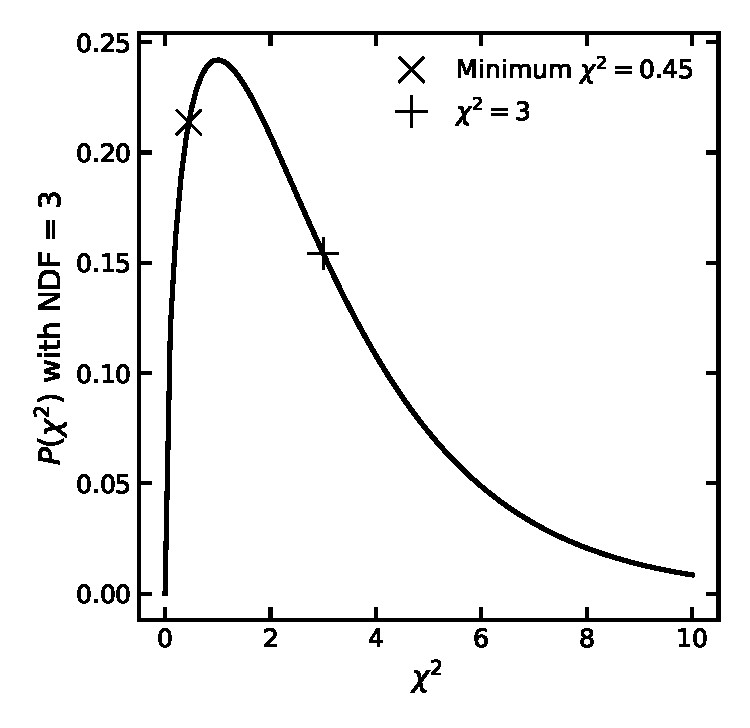
\includegraphics[width=0.5\textwidth]{ch_analysis/min_chi2_final}
    \caption{
        Probability distribution function for the $\chi^2$ distribution
        with 3 degrees of freedom.
        The minimum $\chi^2$ extracted from the fitter
        is marked with an X.
        The expectation value of the minimum $\chi^2$
        for any fit with 3 degrees of freedom is 3,
        which is marked with a $+$.
    }
    \label{fig:chi2_pdf}
\end{figure}

\begin{figure}
    \centering
    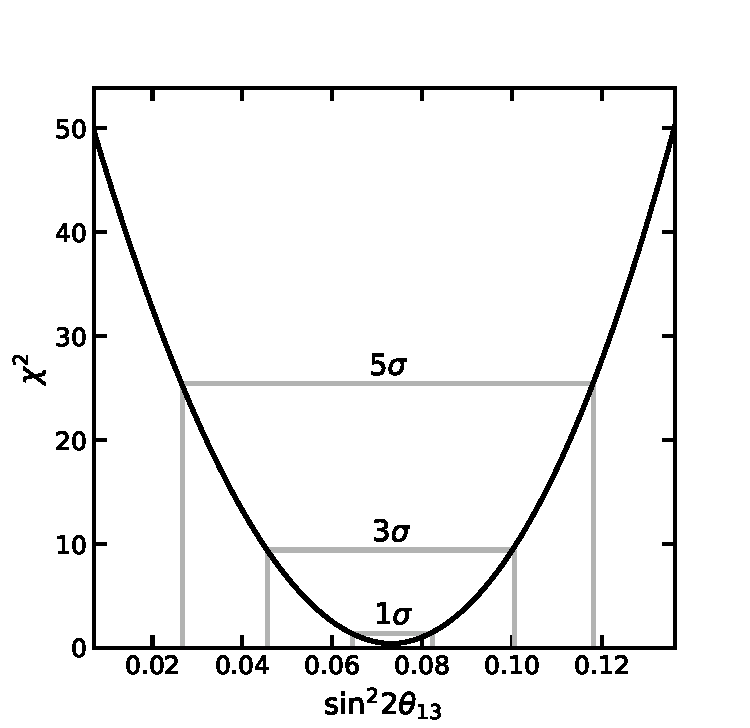
\includegraphics[width=0.5\textwidth]{ch_analysis/chi2_scan_nominal}
    \caption{
        Extracted minimum $\chi^2$ as a function of $\sin^22\thetaot$.
        For each point on the curve, the value of \thetaot{} was fixed
        and the fitter minimized $\chi^2$
        using only nuisance parameters.
    }
    \label{fig:chi2_scan}
\end{figure}

The error budget for this measurement of \thetaot{}
was determined using the subtraction method \cite{nh2016technote}.
This method compares the width of the $\chi^2$ profile
with certain nuisance parameters disabled (fixed at 0)
to the width of the nominal $\chi^2$ profile
to determine the contribution of those paramters
to the final uncertainty of \thetaot{}.
Specifically, the effective uncertainty $\sigma$
was defined as half the range of $\thetaot$ values
producing a $\Delta \chi^2 \leq 1$.
The nominal fit with all nuisance parameters enabled
resulted in an effective uncertainty for \thetaot{} of
\begin{equation}\label{eq:nominal_unc}
    \sigma_\text{all} = \frac{0.0082 + 0.0094}{2} = 0.0088,
\end{equation}
where the two one-sided uncertainties are identical
to those quoted for \thetaot{} in \cref{eq:result}.
The uncertainty due to statistics at the far site was obtained
by disabling all pull parameters
and determining the new range for $\Delta \chi^2 \leq 1$.
This was done without the use of the minimzer since all parameters were specified,
including \thetaot{}.
For all other (systematic) sources of uncertainty $u$,
an effective uncertainty $\sigma^2_{\text{all}-u}$
was obtained by disabling only the nuisance parameters
controlling uncertainty $u$,
and performing a $\chi^2$ scan.
The final uncertainty in $\thetaot$ due to
systematic uncertainty $u$ was
\begin{equation}\label{eq:syst_error_budget}
    \sigma^2_u = \sigma^2_\text{all} - \sigma^2_{\text{all}-u}.
\end{equation}
The modified $\chi^2$ scans are shown in \cref{fig:error_budget_scans},
labeled by the pull parameter category whose impact was tested.
Each source of uncertainty was converted into a relative contribution,
\begin{equation}\label{eq:syst_error_rel}
    f_u = \frac{\sigma^2_u}{\sigma^2_{\text{all}}}.
\end{equation}
The sum of the contributions does not equal unity
due to correlations between the effects of the uncertainties
on \thetaot{}.
Thus a second version, the fractional contribution, was computed as
\begin{equation}\label{eq:syst_error_frac}
    \tilde{f}_u = \frac{\sigma^2_u}{\sum_v \sigma^2_v},
\end{equation}
with the sum taken over all sources of systematic and statistical uncertainty.
The results for both $f_u$ and $\tilde{f}_u$ are
listed in \cref{tab:error_budget}.


\begin{figure}
    \centering
    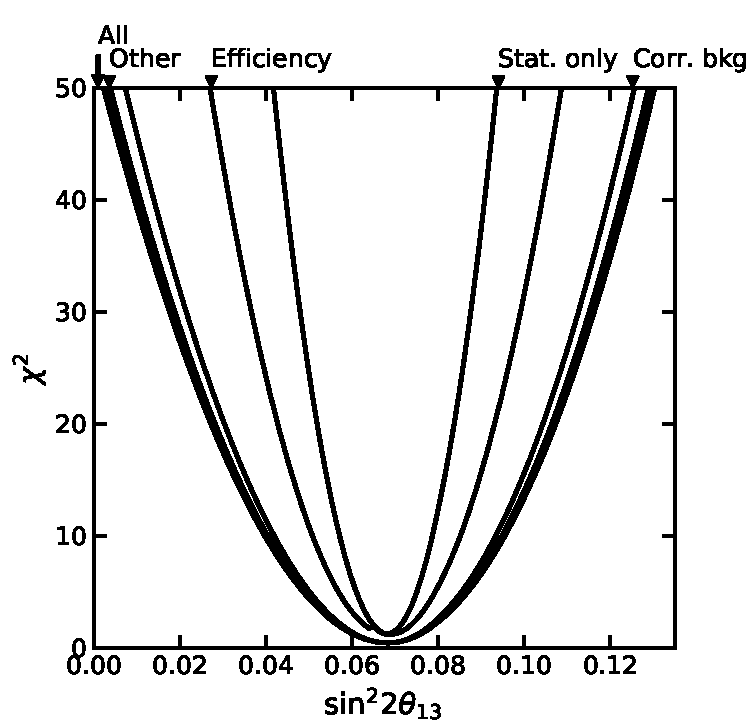
\includegraphics[width=0.5\textwidth]{ch_analysis/error_budget_chi2_scans}
    \caption{
        Scans of $\chi^2$ vs. $\sin^22\thetaot$ with various pull parameters disabled
        in order to determine the contribution of each uncertainty
        to the total uncertainty. (See text for details.)
        The curves labeled ``All'' and ``Stat. only''
        have all pull parameters enabled and disabled, respectively.
        ``Corr. bkg'' includes \li{}/\he{}, fast neutrons, and \amc{}.
        ``Other'' is actually multiple overlapping curves,
        one for each remaining row of \cref{tab:systs}.
        Wider curves indicate a smaller contribution to the total uncertainty.
    }
    \label{fig:error_budget_scans}
\end{figure}

\begin{table}[ht]
    \centering
    \begin{tabular}[t]{lSS}
        \toprule
        Uncertainty source & \parbox[t]{4cm}{
            Relative contribution\\
            $f_u = \left(%
                \sigma^2_u/\sigma^2_\text{all}%
            \right)$ [\%]
        }
        & \parbox[t]{4.2cm}{
            Fractional contribution\\
            $\tilde{f}_u = \left(%
                \sigma^2_u/\sum_v\sigma^2_v%
            \right)$ [\%]
        }
        \\
        \midrule
        Statistics (EH3) & 16.64 & 15.72 \\
        Statistics (EH1 \& EH2) & 1.89 & 1.79 \\
        Detection efficiency & 59.20 & 55.91 \\
        Relative energy scale & 4.08 & 3.85 \\
        Accidental background & 1.29 & 1.21 \\
        \li{}/\he{} background & 14.25 & 13.45 \\
        Fast neutron background & 2.09 & 1.97 \\
        \amc{} background & 0.85 & 0.80 \\
        Reactor power & 5.59 & 5.28 \\
        Input $\theta_{12},\Delta m^2_{21}$, and \dmee{} & 0.01 & 0.01 \\
        \addlinespace
        Total & 105.88 & 100.00 \\
        \bottomrule
    \end{tabular}
    \caption{
        Contribution of each source of uncertainty to the overall uncertainty
        of \thetaot{}.
        Listed values do not sum to the total in each column due to rounding.
    }
    \label{tab:error_budget}
\end{table}





%If the predictions based on different near-hall AD observations agree,
%it can be concluded that the effects due to reactor modeling
%and variation between detectors have been properly accounted for.



%For example, the number of accidental background events in a given near AD
%is estimated to be $N_{\text{acc}}$.
%In the model, this value is subtracted from the total
%observed events in that AD, $N_{\text{obs}}$.
%The expression used to account for the subtraction is,
%in simplified form,

%\begin{equation}
    %(1+\nu_{\text{obs}})N_{\text{obs}} - (1+\nu_{\text{acc}})N_{\text{acc}},
%\end{equation}
%thereby modeling both the statistical uncertainty of the near AD observation
%(as $\nu_{\text{obs}}$ is allowed to change)
%and the systematic uncertainty inherent in
%estimating the number of accidental background events
%(reflected in changes to $\nu_{\text{acc}}$).


